%\documentclass[a4paper,oneside,onecolumn]{article}
\documentclass[journal=nalefd,manuscript=letter]{achemso}
\usepackage{graphicx}
\usepackage{amsmath}
\usepackage{amssymb}
\usepackage{subfigure}
%\usepackage{epstopdf}
%\usepackage{setspace}
%\onehalfspace
%\usepackage{authblk}
%\usepackage[margin=2.3cm]{geometry}

%\geometry{a4paper,left=2.3cm,right=2.3cm,top=2.5cm,bottom=4.5cm}

\usepackage[version=3]{mhchem} % Formula subscripts using \ce{}
\usepackage[T1]{fontenc}       % Use modern font encodings

\newcommand{\nm}{\ensuremath{\,\textrm{nm}}}
\newcommand{\eV}{\ensuremath{\,\textrm{eV}}}
\newcommand{\uM}{\ensuremath{\,\mu\textrm{M}}}
\newcommand{\uW}{\ensuremath{\,\mu\textrm{W}}}
\newcommand{\meV}{\ensuremath{\,\textrm{meV}}}

\author{Aquiles Carattino}
\affiliation[Leiden]
{Huygens-Kamerlingh Onnes, Leiden, The Netherlands}
\author{Veer Keizer}
\affiliation[Leiden]
{Huygens-Kamerlingh Onnes, Leiden, The Netherlands}
\author{Marcel Schaaf}
\affiliation[Leiden]
{Huygens-Kamerlingh Onnes, Leiden, The Netherlands}
\author{Michel Orrit}
\email{orrit@physics.leidenuniv.nl}
\affiliation[Leiden]
{Huygens-Kamerlingh Onnes, Leiden, The Netherlands}

\title{Background-free imaging of gold nanorods through detection of
anti-Stokes emission}

\keywords{Gold nanorods, Plasmon, Imaging, Anti-Stokes, Bio-imaging, Confocal}

\begin{document}
\maketitle
\abstract{This is the abstract}
\section{Introduction}
High-resolution microscopy has become an indispensable tool for studying
biological samples both in vitro and in vivo\cite{Moerner2007}. Organic dyes are
commonly employed to such ends because of their reduced size and high quantum
yield. However this approach is limited to short observation times since
molecules bleach after long irradiation periods. Gold nano-particles on the
other hand are orders of magnitude more stable than organic molecules and are
becoming a standard in many applications including photothermal therapy and
imaging.

Gold nanoparticles do not blink nor bleach, making them ideal candidates for
labeling, tracking and manipulating biological samples over extended periods of
time. Moreover it has been shown that they don't interfere with cells'
functioning, allowing not only in vitro but also in vivo studies. However
compared to organic dyes they exhibit a lower quantum yield, making them
harder to detect in high background scenarios, specially for smaller sizes.

To compensate for the reduced quantum-yield of the particles, several techniques
have been proposed, including two-photon excitation\cite{VandenBroek2013},
photothermal heterodyne detection\cite{Berciaud2006} and interferometric
detection\cite{Ignatovich2006}. All these methods are useful but require
dedicated setups and a high level of expertise to be operated. A method that
allows to image gold nano particles with a high background rejection and that is
readily implementable in current confocal and wide-field microscopes would
provide great benefits for researchers.

Gold nanoparticles exhibit a collective oscillation of surface electrons called
the plasmon. This oscillation exhibits a resonance that is strongly dependent on
the shape of the particles. Spheres with radius roughly between $5$ and $80\nm$
will have a resonance at around $540\,\nm$; more elongated particles, as
nano-rods or bypiramids exhibit resonances that span to even above $800\nm$.
It is important to note that this tuning can be easily achieved at the moment of
the synthesis with a narrow distribution of sizes.

The plasmon is responsible for an enhanced cross section of the particle in a
specific wavelength range but it is also responsible for an enhanced
luminescence emission in the same region. This overlap between the excitation
spectra and the emission spectra of nanoparticles makes them behave in a
complete different way than molecules. If exciting at the absorption maximum
(the plasmon resonance) the majority of the emission will be concentrated in a
narrow spectral region around the excitation. This implies that most of the
luminescence will be blocked by the same filters that prevent direct excitation
light into the detectors. 

It is also possible to excite the particles off-resonance with a
shorter wavelength laser (for instance at $532\,\nm$) and the emission will be
mostly concentrated around to the plasmon resonance. This is the closest picture
to a fluorophore behavior, in which the Stokes-shifted emission can be easily
detected by using a long pass filter. The drawback however, is that the
cross-section of the particle is much smaller at this wavelengths and can only
be compensated by increasing the excitation power; this in turn will also
increase the background intensity.

This work focuses in the exploitation of the anti-Sokes luminescence, which
benefits from the enhanced absorption cross section of the particles, their
stability and narrow emission spectra. Anti-Stokes luminescence in this case
refers to the emission that displays a shorter wavelength than the excitation.
When exciting in resonance with the plasmon, a short pass filter can be
introduced for observing only this emission. The main advantage of this
procedure is that it allows to highly reduce the background arising from
self-fluorescence and Raman-scattering from cells, opening the possiblity to
image and track smaller particles or to use lower excitation powers.

The anti-Stokes emission mechanism can be depicted as follows: an absorbed
photon generates an electron-hole pair with an energy difference equivalent to
the energy of the excitation. After an interaction with the gold lattice, i.e.
with a phonon either the hole gives energy to it or an electron receives energy
from it. This will increase the energy difference between electron and hole; if
they recombine radiatively, the emission will have a shorter wavelength (higher
energy). A schematic of this process can be seen in Figure
\ref{fig:anti-Stokes-process}. The same mechanism can account for the
Stokes-shifted emission, where the only difference is that electron and hole
give energy to the lattice before recombining radiatively.

It has to be kept in mind that the low quantum yield of the particles implies a
low probability of a radiative recombination of electron and holes. Anti-Stokes
emission relies on electron-hole recombination after gaining energy from the
lattice and before any other interaction. Even if this scenario is unlikely,
it is frequent enough as to observe an intensity in the range of $10^3$ counts
per second on an avalanche photodiode with a reasonable excitation power. 

One of the main advantages of the approach presented in this work is its
simplicity at the moment of implementation. Any confocal or wide-field setup
that is capable of exciting nano-particles in resonance can exploit the
anti-Stokes luminescence by adding a proper short-pass filter. Single gold
nanoparticles can be detected even in higher background conditions as a stained
cell, or a highly self-fluorescent sample.

\section{Experimental method}
The core of this work focuses in the employment of a combination of a notch
filter and a  $633\nm$ short pass filter (Semrock) in a home built confocal
microscope as seen in Figure \ref{fig:setup}a. The objective employed was an
oil-immersion Olympus 60X NA 1.4 that allowed a good efficiency in exciting the
particles and collecting their emission. The luminescence signal was then
filtered and was detected by either an avalanche photodiode or a
liquid-nitrogen-cooled CCD-spectrometer (Acton $500\textrm{i}$). Images were
acquired by scanning the sample across the tightly focused laser beam using a
XYZ piezo scanning stage (PI Nano Cube) an example can be seen in Figure
\ref{fig:setup}b.

Gold nanorods were synthesized by following standard seeded-growth
methods\cite{Nikoobakht2003}. The average size of the nanorods was $50\nm\times
20\nm$ and their SPR is located at $630\nm$ in water (refer to the
Supplementary Information for SEM images and bulk extinction spectra of nanorods
as synthesized). Samples were prepared by spin casting a suspension of gold
nanorods into a clean coverslip. 

Lasers with two different wavelengths were employed. A CNI laser with wavelength
of $532\nm$ was used for exciting the transverse plasmon and collect the full
longitudinal plasmon spectrum. Single-particles exhibit a narrow lorentzian
shape as displayed in Figure \ref{fig:setup}c, and therefore this
characterization is useful for discarding clusters of particles. A second laser
(Thorlabs HeNe) with a wavelength of $633\nm$ allowed to excite the particles in
resonance and collect either the Stokes or the anti-Stokes emission.

Figure \ref{fig:emission_peak_position} shows the dependence
of the emission intensity as a function of the plasmon peak position for both
the Stokes and the anti-Stokes. The inhomogeneity observed can be attributed to
a distribution of sizes of the sample (bigger particles will have a bigger cross
section). It is possible to observe, however, that the maximum emission
intensity for the anti-Stokes appears for those particles with the plasmon
slightly blue-shifted from the laser wavelength, while the opposite is observed
for the Stokes emission. This means that there is a trade off between the
excitation efficiency and the collection efficiency: exciting in perfect
resonance is more efficient, but the filters will eliminate the most significant
part of the emission. Exciting off-resonance even if with a smaller
cross-section, improves the collection efficiency. Therefore the particle
described earlier in Figure \ref{fig:spectra_rod} fulfills this condition for
maximum efficiency for the anti-Stokes process.

For proving that the technique is well suited for imaging of particles in
biological conditions, HeLa cells are deposited on top of the nanorod samples.
This allowed to characterize the emission from the particles avoiding their
diffusion out of focus. It may be argued that this condition is not exactly
imaging of rods inside a cell, but resembles very well the condition of imaging in cell
membranes without going into the trouble of the functionalization of the
particles. 

We have also acquired images of nanoparticles under stained cells. This was
achieved by incubating the cells already attached to the coverslips with Atto
647N for approximately half an hour. This set of experiments allows to compare
Stokes and anti-Stokes emission in more unfavorable conditions.

Figure \ref{fig:white-light} shows a typical white light transmission image of
the samples. The high confluency allows to confirm that cells cover uniformly
the entire observed area. In this way we can assure that the studied nanorods
are always below a cell. The higher observed background when working with cells
also is a confirmation of this.


\section{Results and discussion}
Figure \ref{fig:spectra_rod} shows the typical spectra of a gold nanorod under
different conditions. The green curve is the one photon excited luminescence
spectra observed while irradiating with $532\nm$ laser; the full spectrum of the
longitudinal plasmon is clearly observable with it's resonance at $620\nm$. If
the particle is excited at or close to this resonance, the shape of the spectrum
changes drastically: the red curve shows the Stokes shifted emission while
exciting at $633\,\nm$. It was normalized to show the overlap with the curve
obtained with the $532\,\nm$ laser. The blue curve displays the anti-Stokes
emission at shorter wavelengths and the shape, even with the same normalization
constant as for the Stokes case doesn't resemble at all that of the plasmon
resonance. The dashed curves in the Figure correspond to the anti-Stokes and
Stokes emissions without normalization. For this particular nano particle, the
count rate for both types of emissions is comparable, and is also comparable to
the luminescence intensity obtained while exciting at $532\,\nm$. Observing
exclusively the anti-Stokes emission will provide a path to observe gold
nanorods with a great amount of background suppression. 

Figure \ref{fig:shortpass_longpass} shows two raster scans of the same
$15\times15\,\mu m^2$ area of the sample with HeLa cells on top of gold
nanorods. The left image shows the Stokes emission, where a $633\nm$ notch and
$633\nm$ long pass filter were employed. The right image corresponds to the
anti-Stokes emission, where the same notch and a $633\nm$ short pass filter were
employed. In both cases the irradiation intensity was kept at $120\,\mu W$ at
the back aperture of the objective. The same particles are observed with both sets
of filters but the main difference between the two is the background count rate.
In the Stokes image a highly structured background can be observed; we
attribute this emission to self-fluorescence of the cell. The anti-Stokes
image shows a much flatter background and highly distinguishable single
particles. Both images display the absolute count rate obtained without any
further dark count subtraction. 

Figure \ref{fig:distribution_pixels} shows the distribution of pixel intensities
in both images. The Stokes image shows a distribution of values centered around
$55$ counts/$10\textrm{ms}$, while the anti-Stokes shows a maximum at $1$
count/$10\textrm{ms}$ that roughly coincides with the dark counts of the
detector. This already is a big indication that the majority of the background
in the anti-Stokes case arises from the detector and not from the sample. This
is however not true in the entire image. The region close to the origin ($0,0$)
shows a slightly higher emission in both cases. This may be due to to an
anti-Stokes Raman emission from the cell itself and that can not be filtered out
with a short pass filter.

To prove the usefulness of the method in situations with even higher
backgrounds, we incubated the cells with a solution of Atto 647n. This staining
of the cell, even if not specific, results in a similar situation that what
would be obtained in the case of labeling of particular organelles or the entire
cell membrane. The dye was chosen because its absorption maximum is close to
$633\nm$, the excitation wavelength we were employing in these experiments. 

Figure \ref{fig:Stokes_AS_with_dye} shows two raster scans of the samples
described above. The left shows the anti-Stokes result, in which
single-particles are clearly distinguishable. The right one shows the Stokes
emission, in which at most one particle can be clearly distinguished from the
background. The distribution of intensities in Fig. \ref{fig:hists_dye}
show a clear change as compared to the situation without dye. The anti-Stokes
maximum is closer to $5$ counts/$10$ms, higher than the dark counts of the
detector. The Stokes emission, on the other hand shows a distribution centered
around $2000$ counts/$10$ms, one order of magnitude higher than the observed
without the dye. 

These results indicate that the Stokes imaging deteriorates much faster than the
anti-Stokes in the presence of emitting molecules both from the cell itself or
from the dye added a posteriori. The images show regions with higher emission
intensities in both configurations, most probably due to a higher concentration
of dye in particular regions of the cell. At much higher concentrations than
the ones employed in this work, the dye has also shown anti-Stokes emission at
rates even higher than the particles, meaning that a balance has to be obtained
to still be able to detect the particles.

Figure \ref{fig:power_intensity}a shows the dependence of the acquired
luminescence and the background as a function of excitation power for both the
Stokes and anti-Stokes emissions of a particle below cells without dye. For the
Stokes (red curves) a linear increase in signal is accompanied by an increase in
background, hence the ratio saturates even for low powers. The anti-Stokes
(blue-curves) however shows a much steeper increase of the signal as compared to
the background. This means that for excitation powers high enough, the
signal-to-background ratio is higher for the anti-Stokes emission.

Figure \ref{fig:power_intensity}b shows the same curves but in the case where
the cells were stained. It can readily be seen that in the Stokes case the
particle is barely above the signal arising from the background, while the
anti-Stokes shows an enhanced contrast. We attribute the increase in the
background to the anti-Stokes emission from the dye itself; it is of no surprise
that a molecule absorbing laser light exhibits this emission at room
temperature. 

Even if the signal-to-background ratio seems to increase with higher laser
powers, this can't be extrapolated further than the results here presented.
It is known that gold nano rods reshape at elevated temperatures. Increasing
irradiation intensity, implies increasing the temperature of the particles
that would slowly start to reshape into spheres. For high-NA objectives like the
one employed in this work, a rule of thumb is not to surpass $150\,\muW$ at the
back aperture to prevent reshaping.

\section{Conclusions}
In this work we have proved that the anti-Sokes emission arising from the
excitation in (or close to) the plasmon resonance of a gold nanorod can be
exploited to image them in biological conditions. The comparison between the
Stokes and anti-Stokes was possible by using immobilized particles, but this
work proves that the same technique can be employed for imaging particles in
fixed cells, for example. 

Extending this technique to wide-field should be possible considering the
laser powers employed in this work. EMCCDs provide enough gain as to easily
detect single nanoparticles, while at the same time the background is considerable low
(or negligible for low powers). This extension of the technique would provide a
way of doing tracking at higher framerates than achivable by confocal imaging. 

The lower countrate of the anti-Stokes as compared to the Stokes emission is
however a drawback. For doing localization it is usually better to have a higher
countrate than a better signal-to-background ratio. On the other hand this work
shows the possibility of observing particles in less favorable conditions, as
may be a stained cell, or smaller particles which will have smaller cross
sections but still be brighter than the background.

\begin{figure}[p]
 \centering 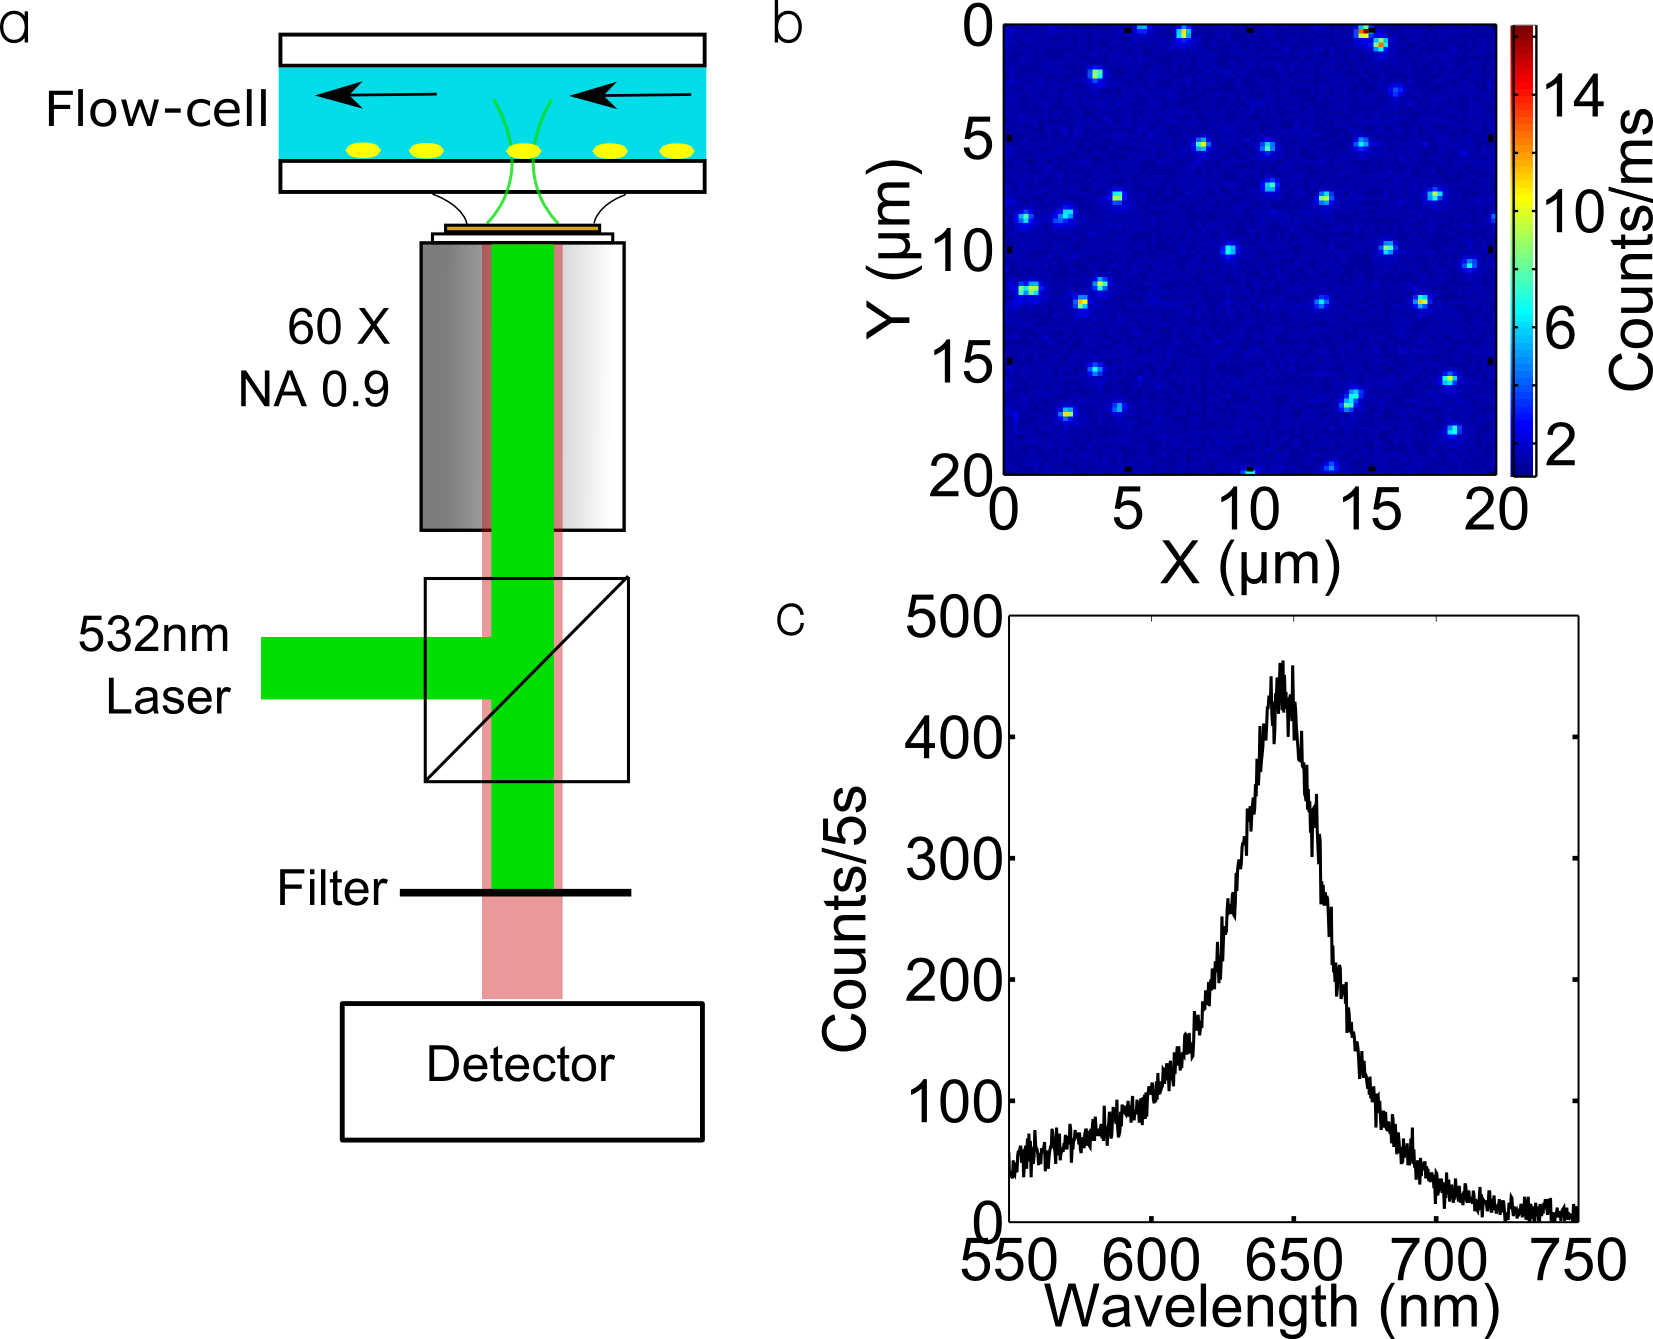
\includegraphics[width=0.45\linewidth]{Figures/01_Setup/setup_1.png}
 \caption{Experimental setup and examples of observations. a) Simplified
 schematic of the confocal microscope employed during the measurements. b) A
 typical 1-photon luminescence raster scan of the sample immersed in
 water c) luminescence spectrum of a single rod.}
 \label{fig:setup}
\end{figure}

\begin{figure}[p]
\centering
	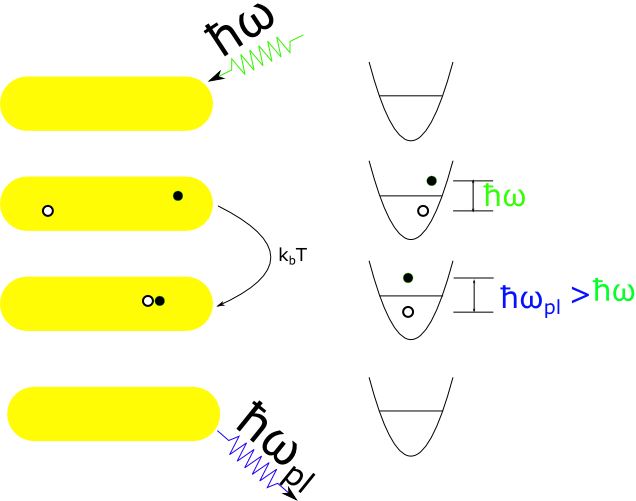
\includegraphics[width=0.4\linewidth]{luminescence_all_AS.png}
	\caption{Schematic of the anti-Stokes luminescence arising from a single gold
	nanorod. The emission with a higher energy than the excitation energy can be
	explained by an interaction between the electron and the phonons in the metal}
	\label{fig:anti-Stokes-process}
\end{figure}

\begin{figure}[p]
\centering
	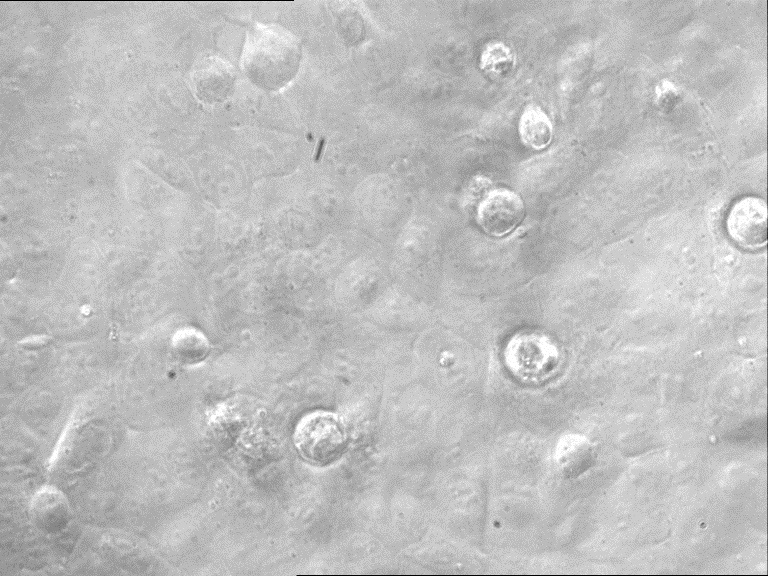
\includegraphics[width=0.4\linewidth]{U2OS_12.jpg}
	\caption{White light transmission image of the sample with cells deposited on
	top of the rods. It is possible to observe that they cover entirely the
	observed region without spacing in between them. The spherical cells seen out
	of focus are cells that can't attach to the glass, remaining with that shape.}
	\label{fig:white-light}
\end{figure}

\begin{figure}[p]
\centering
	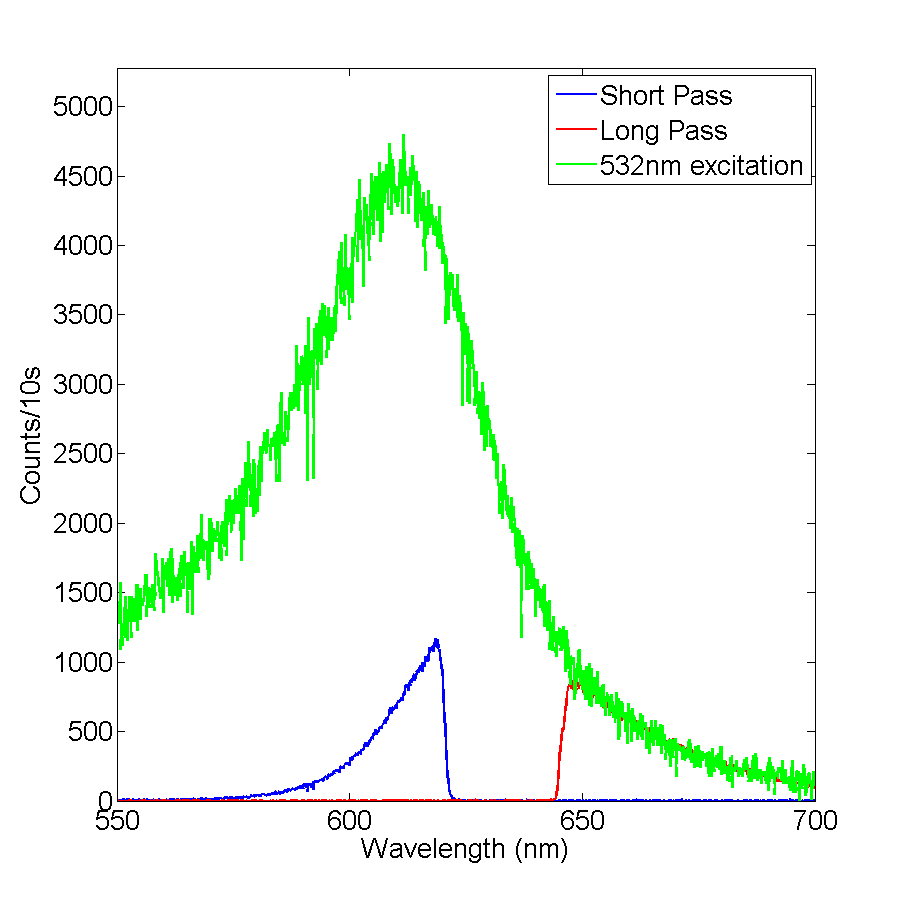
\includegraphics[width=0.4\linewidth]{3_Curves.png}
	\caption{Luminescence spectra of a single gold nanorod excited with a $532\nm$
	laser (green curve). The Stokes emission after excitation with a $633\nm$
	HeNe laser is the red curve and the blue curve corresponds to the anti-Stokes
	emission. These last two curves were normalized such that the Stokes emission
	overlaps the spectrum obtained with the $532\nm$ laser.}
	\label{fig:spectra_rod}
\end{figure}



\begin{figure}[p]
\centering
	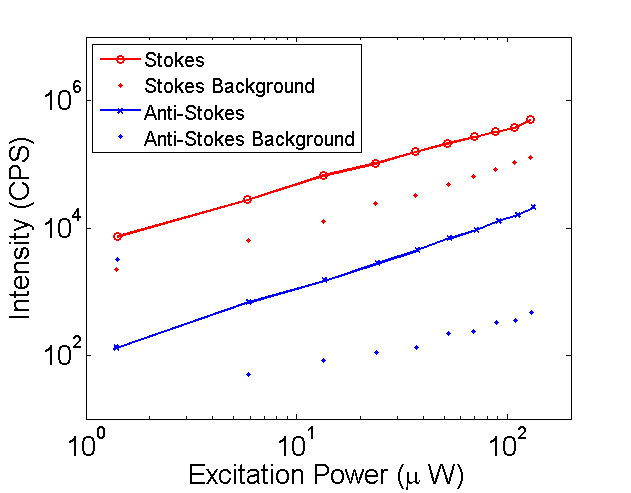
\includegraphics[width=0.4\linewidth]{plce_4_bis.png}
	\caption{Emission intensity as a function of excitation intensity for: the
	Stokes emission (of both the particle and the background) and the anti-Stokes
	emission. A particle with the plasmon close to the laser line was chosen as to
	avoid favouring one or the other emission.}
	\label{fig:power_intensity}
\end{figure}

\begin{figure}[p]
\centering
	\subfigure{%
	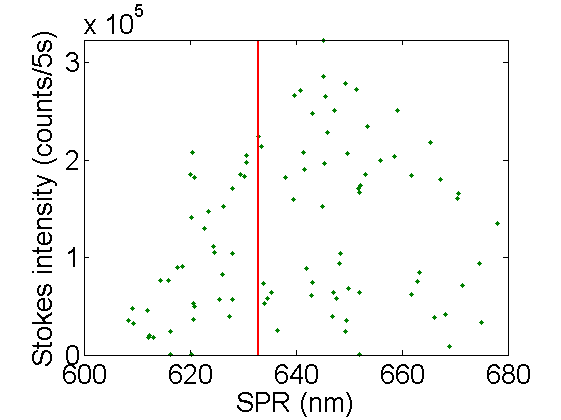
\includegraphics[width=0.4\linewidth]{intensity_vs_plasmon_LP.png}}
	\subfigure{%
	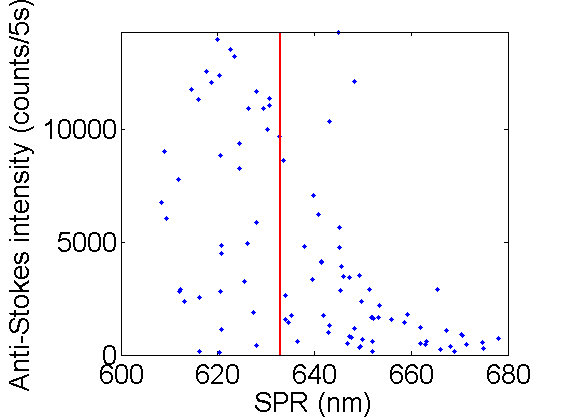
\includegraphics[width=0.4\linewidth]{intensity_vs_plasmon_SP.png}}
	\caption{Emission intensity as a function of plasmon peak position for the
	Stokes (a) and anti-Stokes (b) sides. The spread in intensities for similar
	peak position can be attributed to variations in sizes or different
	orientations of the rods in a non perfectly circularly polarized beam.}
	\label{fig:emission_peak_position}
\end{figure}

\begin{figure}[p]
\centering
	\subfigure{%
	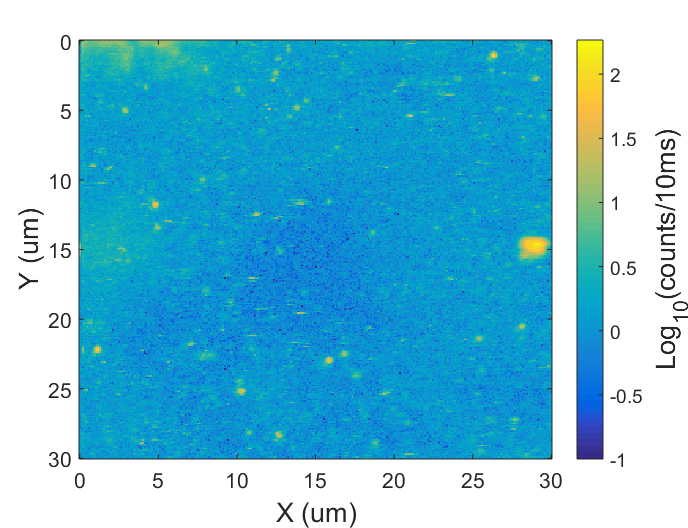
\includegraphics[width=0.4\linewidth]{Figures/03_Stokes_AS/anti_stokes.png}}
	\subfigure{%
	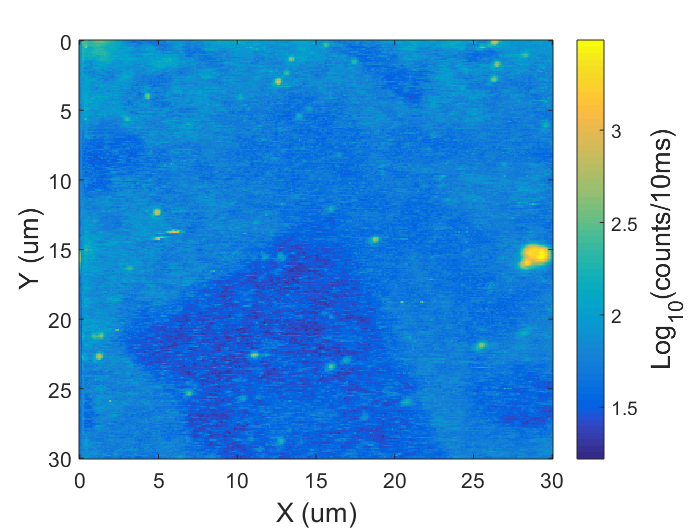
\includegraphics[width=0.4\linewidth]{Figures/03_Stokes_AS/stokes.png}}
	\caption{Raster scan using a long pass filter (a) and a short pass filter (b).
	The same rods can be observed; it has to be noted that not necessarily the
	brightest in the Stokes emission will be the brightest in the anti-Stokes.}
	\label{fig:shortpass_longpass}
\end{figure}

\begin{figure}[p]
\centering
	\subfigure{%
	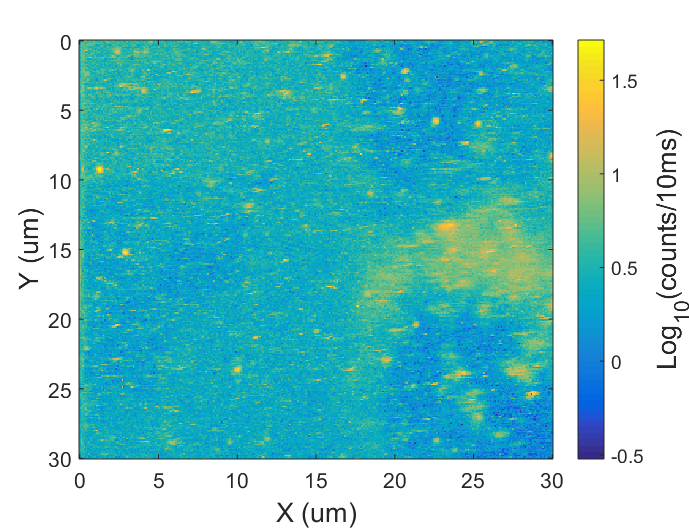
\includegraphics[width=0.4\linewidth]{Figures/04_Soktes_AS_with_dye/anti_stokes.png}}
	\subfigure{%
	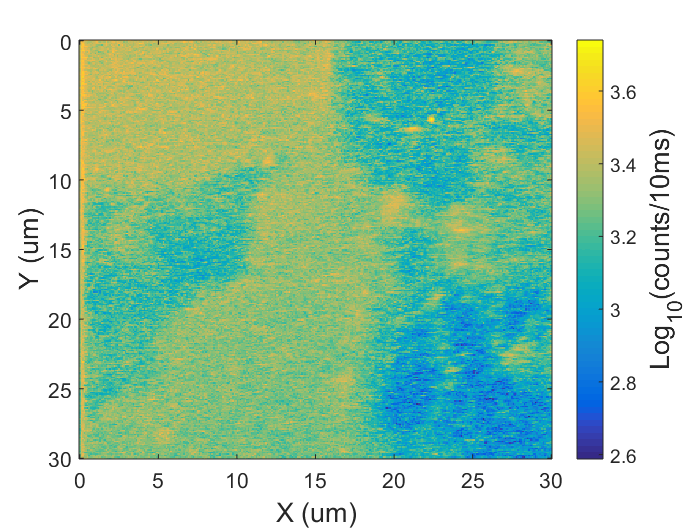
\includegraphics[width=0.4\linewidth]{Figures/04_Soktes_AS_with_dye/stokes.png}}
	\caption{Raster scan using a long pass filter (a) and a short pass filter (b).
	The same rods can be observed; it has to be noted that not necessarily the
	brightest in the Stokes emission will be the brightest in the anti-Stokes.}
	\label{fig:Stokes_AS_with_dye}
\end{figure}

\begin{figure}[p]
\centering
	\subfigure{%
	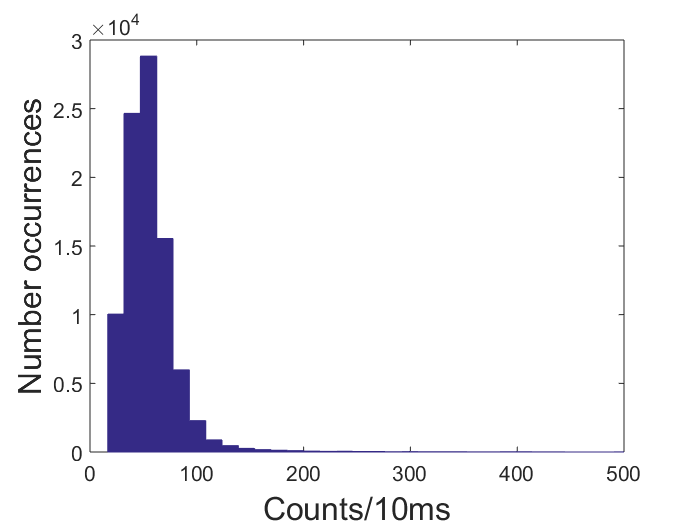
\includegraphics[width=0.4\linewidth]{Figures/03_Stokes_AS/hist_stokes.png}}
	\subfigure{%
	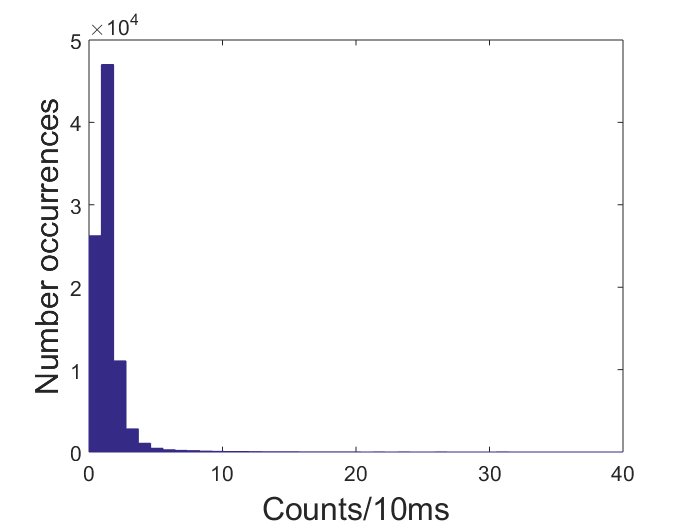
\includegraphics[width=0.4\linewidth]{Figures/03_Stokes_AS/hist_anti_stokes.png}}
	\caption{Pixel intensity distribution for anti-Stokes and Stokes emission.}
	\label{fig:distribution_pixels}
\end{figure}
\end{document}
